% !TEX encoding = UTF-8
% !TEX TS-program = pdflatex
% !TEX root = ../tesi.tex

%**************************************************************
\chapter{Progettazione e realizzazione} %TODO e codifica
\label{cap:progettazione}
%**************************************************************

\intro{Il capitolo corrente ha lo scopo di illustrare l'architettura del plugin nel  dettaglio con il supporto di diagrammi e le scelte progettuali effettuate.}\\

\section{Procedura di lavoro}
Inizialmente per capire il funzionamento di un plugin Maven e delle API RESTful del server documentale (Confluence), è stato dedicato del tempo allo studio autonomo.
Successivamente è stato sviluppato un Proof of Concept al fine di mettere in pratica quanto appreso dalla teoria.
Il prototipo consisteva in un semplice plugin Maven che effettuava delle stampe e delle chiamate REST ad un server creato al momento con Meecrowave.
Questo prototipo è successivamente cresciuto ed è stato ampliato e modificato per poter interagire con il plugin \emph{Docs} di Confluence.
Ciò ha permesso di comprendere il caricamento di materiale su \emph{Docs} ed ha consentito di effetture la scelta delle librerie Java più adatte per il prodotto finale.


%**************************************************************
\section{Tecnologie e librerie utilizzate}
\label{sec:tecnologie-strumenti}

In questa sezione viene data una panoramica delle tecnologie e librerie principali utilizzate.
Esse sono state scelte dalla candidata in concomitanza con gli sviluppatori DevOps senior dell'azienda.


\subsection{JavaX}
JavaX è un package di estensioni standard per il linguaggio Java.
Le estensioni che include sono numerose; quelle usate per la realizzazione del prodotto sono:
\begin{itemize}
    \item \bd{javax.annotation}: per le annotazioni  \texttt{Nonnull} e  \texttt{Nullable}, richieste secondo la politica aziendale, in modo da segnalare gli elementi che possono essere nulli o meno;
    \item \bd{javax.ws.rs.core}: per la creazione di risorse relative ai servizi
    RESTful, utili per il client al momento della comunicazione con Confluence;
    % Low-level interfaces and annotations used to create RESTful service resources
    \item \bd{javax.xml.bind.annotation}: per la trasformazione automatica di JSON in oggetti Java, utile per convertire i messaggi mandati da Confluence in oggetti facilmente manipolabili dal plugin.
\end{itemize}


\subsection{Codehaus Plexus}
Codehaus Plexus è una collezione di componenti usata da Apache Maven.
Le librerie adottate per il progetto sono:
\begin{itemize}
    \item \bd{org.codehaus.plexus.archiver}: per l'archiviazione della documentazione;
    \item \bd{org.codehaus.plexus.util}: per utilità varie, adatte per la scrittura su file.
\end{itemize}


\subsection{Maven}
Maven è la tecnologia centrale del prodotto.
Di essa sono state utilizzate numerose classi, ma i package principali sono:
\begin{itemize}
    \item \bd{org.apache.maven.plugins.annotations}: per le annotazioni relative ai plugin Maven, quali per esempio \texttt{Mojo} per identificare un \emph{goal},  \texttt{Paremeter} per segnalare un parametro della configurazione, ecc;
    \item \bd{org.apache.maven.plugin}: per le eccezioni che può lanciare un plugin Maven;
    \item \bd{org.apache.maven.project}: per accedere alle informazioni del progetto (quali nome e versione);
    \item \bd{org.apache.maven.settings}: per decriptare le credenziali provenienti dal file ``settings.xml''.
\end{itemize}


\subsection{Jersey} %aveva tanta documentazione rispetto ad altri client
Jersey è un framework opensource per lo sviluppo di servizi web RESTful in Java.
All'interno del progetto è stata una parte focale perché utilizzato per la creazione del client:
\begin{itemize}
    \item \bd{com.sun.jersey.api.client}: per il client che effettua le chiamate verso Confluence;
    \item \bd{com.sun.jersey.api.client.config}: per la configurazione iniziale del client.
\end{itemize}



%**************************************************************
\section{Diagramma dei package} %TODO da rifare
\label{sec:diagramma-package}
\begin{figure}[H]
    \centering
    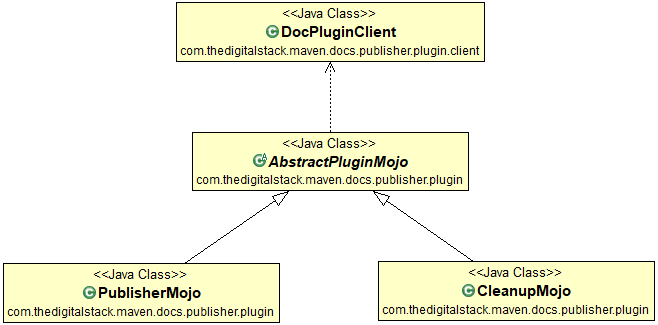
\includegraphics[width=0.8\textwidth]{immagini/PackageDiagram.png}\\
    \caption{Diagramma dei package}
\end{figure}
Le classi principali del \emph{Maven documentation publisher plug-in} sono i \emph{mojos} di Maven e il client.
Un \emph{mojo} è un \emph{goal} esguibile in Maven, ovvero la classe che concretamente realizza lo scopo prefissato.
I \emph{mojos} appartengono al package Java \texttt{com.thedigitalstack.maven.docs.publisher.plugin} e il client al sub-package\\ \texttt{com.thedigitalstack.maven.docs.publisher.plugin.client}.
Tra loro è possibile identificare due classi fondamentali: PublisherMojo e CleanupMojo.
Entrambe sono \emph{mojos} di Maven e perciò determinano \emph{goal} differenti.
Alcuni metodi che riguardano il client e le impostazioni del server sono uguali, per questo motivo esiste una classe padre e un riferimento a DocPluginClient.
DocPluginClient svolge le operazioni lato client ed è l'unico oggetto che comunica direttamente con Confluence.



%**************************************************************
\section{Diagrammi delle classi}
\label{sec:diagrammi-classi}

\begin{figure}[H]
    \centering
    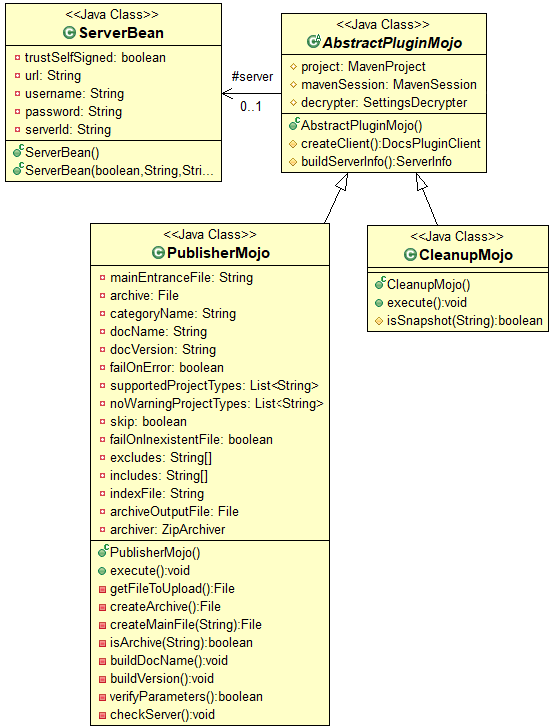
\includegraphics[width=0.95\textwidth]{immagini/mojo-gerarchy.png}\\
    \caption{Diagramma delle classi relativo alla gerarchia principale del plugin}
\end{figure}

\txt{PublisherMojo} realizza la pubblicazione della documentazione su Confluence, per questo motivo, il suo \emph{goal} è nominato \emph{publish} e la fase del ciclo di vita Maven relativo al progetto è package di default.

%TODO sistemare tabella con i parametri
\begin{table}[H]
    \centering
    {\def\arraystretch{1.7}
    \begin{tabularx}{\textwidth}{XXXX}
        \rowcolor{beautyblue} \textbf{Parametro} & \textbf{Necessario} & \textbf{Descrizione} & \textbf{Valore di default} \\\toprule
        archive & Sì & Documentazione da pubblicare & - \\
        Di qualità & 11 & 1 & 3 \\
        Di vincolo & 11 & 0 & 5
        \\\bottomrule
    \end{tabularx}}
    \caption{Riepilogo dei requisiti}
\end{table}

\txt{CleanupMojo} si occupa dell'eliminazione completa delle pagine \emph{doc} contenenti SNAPSHOT.
Ciò significa tutta la documentazione la cui versione comprende il qualificatore ``-SNAPSHOT''.
Per questo motivo, il \emph{goal} relativo si chiama \emph{cleanup} e non è specificata nessuna fase del ciclo di vita di un progetto Maven.
Esso non richiede altri parametri in uso dall'utente: fa semplicemente affidamento sul method \txt{isSnapshot(String)} per comprendere se il titolo valutato è un ``-SNAPSHOT''.

PublisherMojo e CleanupMojo estendono \txt{AbrasctPluginMojo}.
Questa classe astratta estende \txt{AbrasctMojo} (la classe astratta base di qualunque \emph{mojo} Maven) e definisce i metodi in comune ad entrambi, come per esempio \txt{createClient()} per l'inizializzazione del cient, lasciando implementare il metodo \txt{execute()} alle sottoclassi.

AbstractPluginMojo fa uso di un oggetto di tipo\txt{ServerBean} che contiene le informazioni richieste per connettersi al server Confluence, come per esempio la URL e le credenziali dell'utente.
Per lo più esso richiede un booleano (\txt{trustSelfSigned}) per determinare se il certificati SSL sono eccettati, e una stringa \txt{serverId} nel caso l'utente volesse permettere di ricavare le credenziali dal file ``settings.xml''.



% -------------------------

L'utente può scegliere della documentazione:
	\begin{itemize}
		\item \bd{nome}: alternativamente preso dal nome del progetto o \emph{artifactId};
		\item \bd{versione}: alternativamente preso dalla versione del progetto.
	\end{itemize} 
Il titolo della pagina \emph{doc} viene costruito dalla congiunzione di nome e versione.
Vengono riportati qui di seguito alcuni esempi:
	\begin{enumerate}
		\item docName= Quickstart Doc, docVersion= 2019, project name= Quickstart Vogella project, project version= 2.1.1-SNAPSHOT, artifactId= quickstart
		\item project name= Quickstart Vogella project, project version= 2.1.1-SNAPSHOT,  artifactId= quickstart
		\item docVersion=2018, project version= 2.1.1-SNAPSHOT,  artifactId= quickstart
	\end{enumerate}

	\begin{figure}[H]
		\centering
		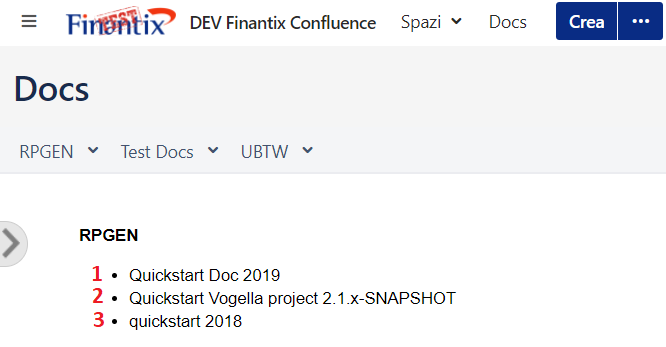
\includegraphics[width=0.7\textwidth]{immagini/DocsExamples.png}\\
		\caption{Screenshot di un esempio di Docs Plug-in}
	\end{figure}

% ---------------------------



\begin{figure}[H]
    \centering
    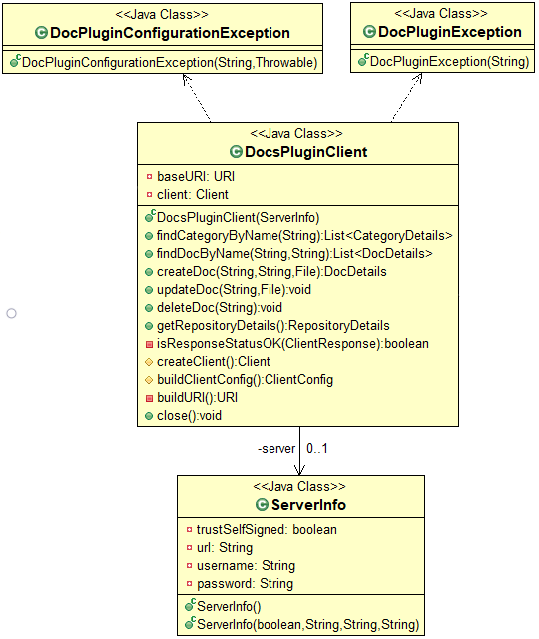
\includegraphics[width=0.9\textwidth]{immagini/client.png}\\
    \caption{Diagramma delle classi relativo al client}
\end{figure}

Il client è creato da AbstractPluginMojo ed è un oggetto di tipo \txt{DocsPluginClient}.
Questa classe fornisce tutto il necessario per creare ed usare un'istanza del client Jersey: riceve le informazioni per la configurazione da ServerInfo (un semplice Java bean simile a ServerBean) e produce la directory di base richiesta per svolgere qualunque tipo di chiamata REST.
I metodi che compiono delle chiamate REST sono:

\begin{table}[H]
    \begin{paddedtablex}[1.7]{\textwidth}{XcX}
        \rowcolor{beautyblue}\textbf{Nome} & \textbf{Richiesta} & \textbf{Descrizione} \\
        \toprule

        \txt{findCategoryByName(String categoryName)} & \bd{GET} & Ritorna una lista di categorie esistenti, il cui nome coincide con la stringa data \\
        \txt{findDocByName(String categoryId, String docName)} & \bd{GET}  & Ritorna una lista di doc esistenti all'interno di una categoria esistente e i cui nomi coincidono con la stringa data \\
        \txt{createDoc(String categoryId, String docName, File docArchive)} & \bd{PUT} & Crea la pagina doc all'interno di una categoria esistente, con l'archivio e il nome dato \\
        \txt{updateDoc(String docKey, File docArchive)} & \bd{POST} & Aggiorna la pagina doc identificata dalla \txt{docKey} data, con l'archivio dato \\
        \txt{getRepositoryDetails()} & \bd{GET} & Ritorna tutti i dettagli relativi alla repository: tutte le categorie e i doc esistenti \\
        \txt{deleteDoc(String docKey)} & \bd{DELETE} & Elimina la pgina doc relativa alla \txt{docKey} data \\

        \bottomrule
    \end{paddedtablex}
    \caption{Metodi di DocsPluginClient che compiono chiamate REST}
\end{table}




% ----------- da tradurre ----------

DocsPluginClient class provides all the necessary to create and use an instance of Jersey client. It receives the configuration information by ServerInfo (a simple bean class similar to ServerBean) and realizes the base directory required by every REST call. Primary methods which performs REST calls are:

Mostly everyone of these methods can throw a DocPluginException when the client response received is unexpected because something went wrong. Another exception that DocsPluginClient can throw is DocPluginConfigurationException: a RuntimeException which can occur during client building.




\begin{figure}[H]
    \centering
    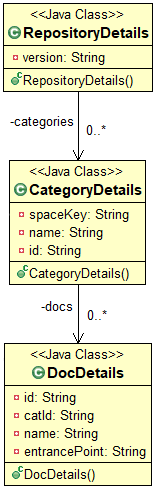
\includegraphics[width=0.26\textwidth]{immagini/details.png}\\
    \caption{Diagramma delle classi relativo ai dettagli di ogni componente del plugin Confluence}
\end{figure}

\section{Diagrammi di sequenza}
\label{sec:diagrammi-sequenza}

\begin{figure}[H]
    \centering
    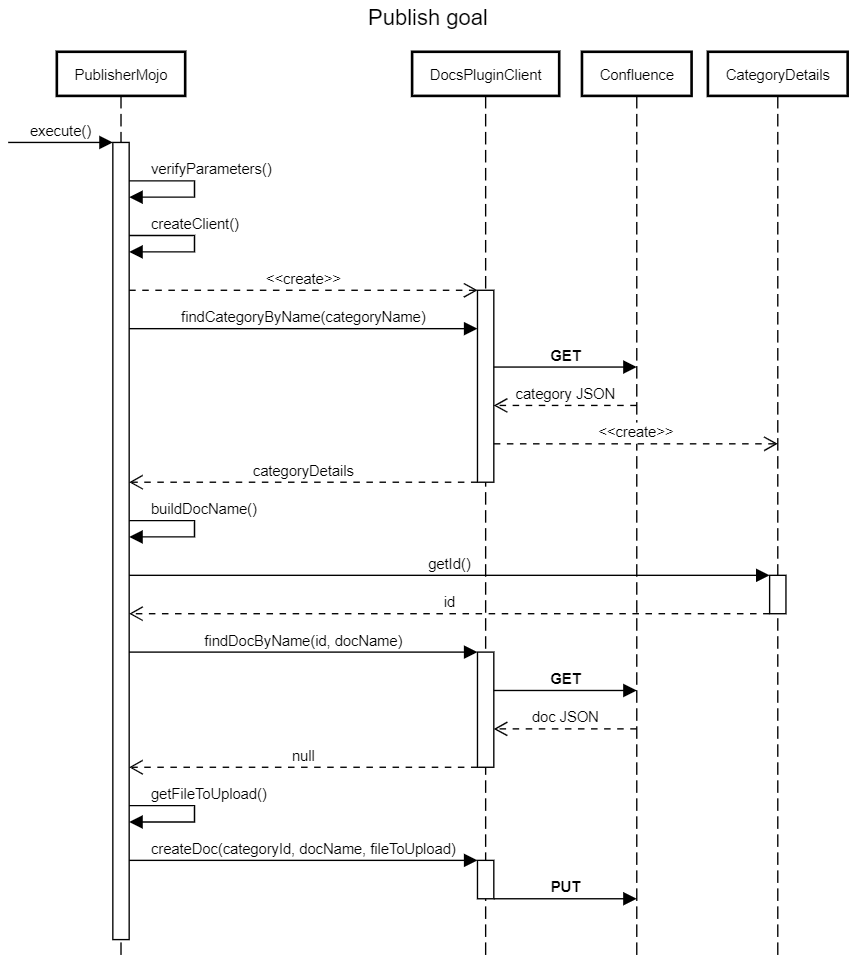
\includegraphics[width=\textwidth]{immagini/CreateDocSequence.png}\\
    \caption{Diagramma di sequenza relativo al goal \emph{publish}}
\end{figure}

\begin{figure}[H]
    \centering
    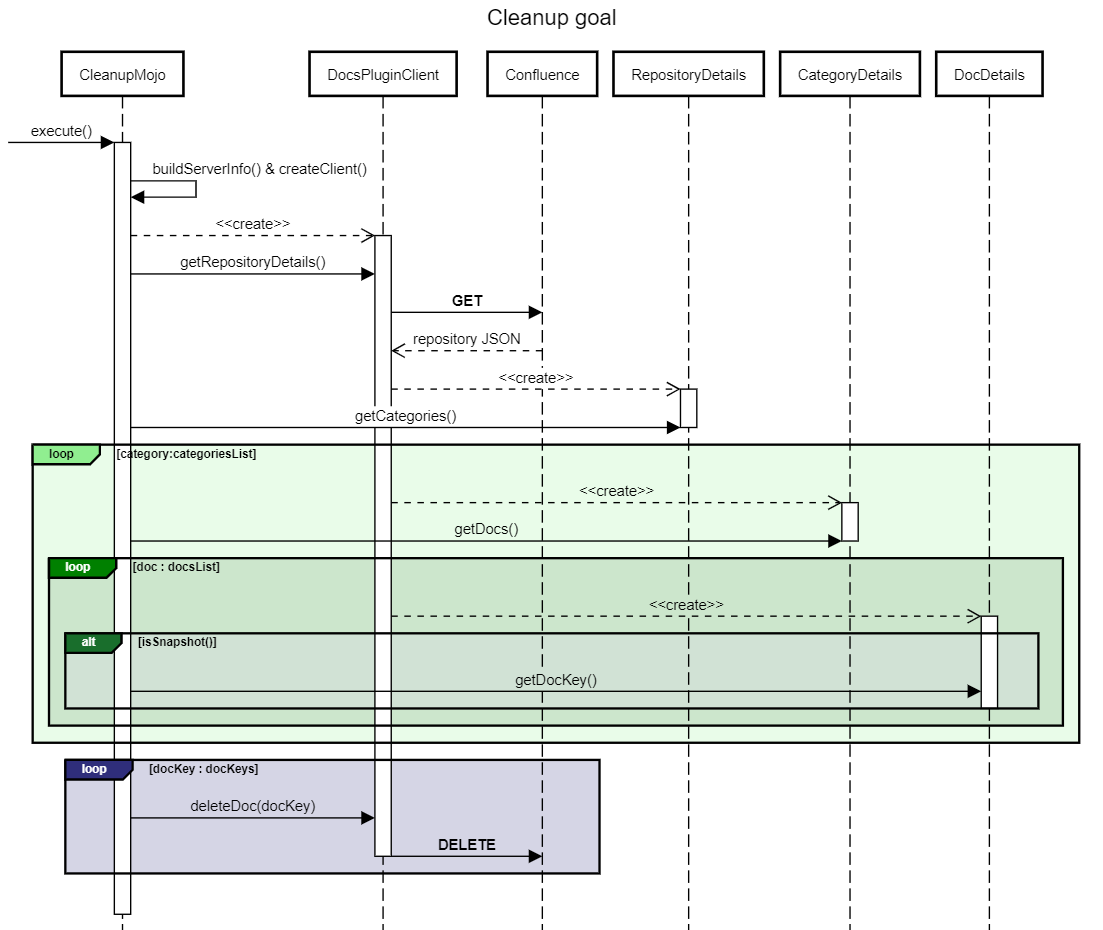
\includegraphics[width=\textwidth]{immagini/SequenceCleanupConfluence.png}\\
    \caption{Diagramma di sequenza relativo al goal \emph{cleanup}}
\end{figure}

%**************************************************************
% \section{Ciclo di vita del software}
% \label{sec:ciclo-vita-software}

%**************************************************************
% \section{Progettazione}
% \label{sec:progettazione}

% \subsubsection{Namespace 1} %**************************
% Descrizione namespace 1.

% \begin{namespacedesc}
%     \classdesc{Classe 1}{Descrizione classe 1}
%     \classdesc{Classe 2}{Descrizione classe 2}
% \end{namespacedesc}


%**************************************************************
\section{Design Pattern utilizzati}

\subsection{Template Method}

%**************************************************************
% \section{Codifica}
